\chapter{Konzeption und Implementierung}

Das neue Konzept, das in diesem Kapitel erklärt wird, beinhaltet die Migration von Datenbanken von der alten webbasierten Software zur neuen Software, die auf Umbraco CMS basiert. Die Funktionalitäten müssen gleich bleiben.  
Das Projekt unterteilt sich in zwei großen Pakete – Paket A und Paket B.
Im ersten Paket wird die Verwaltung des Frontends aufgebaut. Das Ziel ist maximale Flexibilität für den Website-Besitzers und durch einfache Tätigkeiten, bestimmte Zwecke zu erfüllen. Man soll in diesem Bereich den Inhalt der Webseite editieren, ändern und erweitern können. 
Umbraco verfügt über sogenannte „Grids“. Sie dienen dazu, dass man das Design der Seite manipulieren und auch die schon besprochenen Möglichkeiten ausnutzen kann. 
Es werden auch eigene Makros benutzt, in den ein Quellcode der SHOP – Komponenten hingeschrieben wird. Somit kann der Auftraggeber Makros in beliebigen Teilen der Seiten einfügen. Umbraco – Forms werden als Formulare benutzt, damit man selber die Felder einordnen kann.
Beide Pakete werden als Startknoten aus einer Umbraco-Instanz heraus verwaltet. 
Paket B ist als Kern der Seite aufgebaut. Das ist eigentlich das Online-Bestellsystem. Hier ist es wichtig, dass eine unkompliziert bedienbare, reibungslose und flexible Umgebung aufgebaut wird. Das System besteht aus drei Hauptkernen:
 
\begin{itemize}	
	\item Bestellsystem
	\subitem Kundenverwaltung (Anmeldung, Kundenbereich, Kommunikation)
	\subitem Artikelverwaltung
	\subitem Auftragsverwaltung
	\item E-Mail-Verwaltung
	\subitem E-Mail-Vorlagen anlegen, editieren, löschen
	\item Umsatzerfassung
	\subitem Umsatzübersicht nach Monat und Jahr
\end{itemize}

\section{Aufbau vom Umbraco}

Wie oben schon erklärt wurde, ist Umbraco \cite{Wahlberg2011} ein Content Management System, das flexibel und Benutzerfreundlich ist. Für ein besseres Verständnis, worum es geht, wird es in diesem Unterkapitel erläutert. 

Das User Interface von Umbraco ist auf drei Teile unterteilt. Erste Teil ist Hauptfunktion bzw. Setcion. Dort befinden sich die Hauptoptionen: Content, Media. Settings, Developer, Users, Members, Forms.
Damit ein klarer Unterschied zwischen „Member“ und „User“ gemacht wird, werden die beiden Begriffe erklärt. „User“ ist jemand, der Zugriff zu „Umbraco-Backoffice“ hat und dort bestimmte Rechte hat. 

Ein Member wird von Umbraco für die Registrierung und Authentifizierung eines externen Besuchers benutzt. Das sind Leute, die nur Front-End benutzen dürfen. 
Man kann auch eine „Custom Setcion“ erstellen, womit wir uns im weiteren Kapitel beschäftigen. 

Der nächste Teil ist die Unternavigation oder auch Tree genannt. Alle Unteroptionen stehen dort. Jede Hauptfunktion hat ihre eigenen Unteroptionen.
Zugehörige Funktionalitäten der Unteroptionen (Trees) werden betrachtet. Die Abbildung \ref{fig:UmbracoFunktionalitaet} stellt das Funktionsprinzip von Umbraco \cite{UmbracoHQ2018Backofficeoverview}.

\begin{figure}[h]
	\centering
	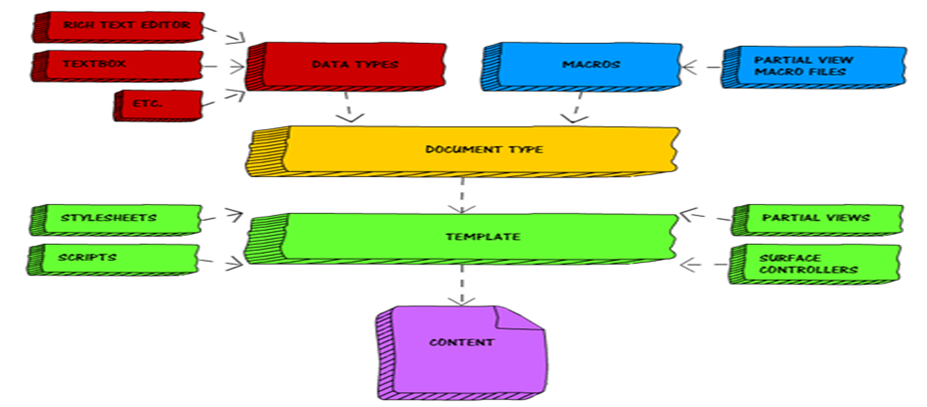
\includegraphics[width=1\linewidth]{Graphics/umbracoAufbau.png}
	\caption[Umbraco Backoffice]{Funktionalität vom Umbraco-Backoffice\\Quelle: http://droom.biz/umbraco-architecture-diagram/e-member-to-rule-them-all-umbraco-architecture-diagram/
	}
	\label{fig:UmbracoFunktionalitaet}
\end{figure} 

\begin{itemize}	
	\item\textbf{Trees vom Content-Section:} In diesem Tree befinden sich alle Seiten, die im Website Front-End erschienen werden können. Dort steht auch Recycle Bin, oder auch Papierkorb genannt. So kann man die gelöschte Seite zurücksetzen. 
	\item\textbf{Trees von der Media-Section:} Hier stehen alle Videos und Bilder zur Verfügung.
	\item\textbf{Trees vom Settings-Section:} In diesem Tree befindet sich Moglichkeiten CSS, JavaStript, Document Types und zugehörige Templates. PatialView ist auch dort. Es hat eine Übertragungsfunktion von Backend zum Frontend.
	\item\textbf{Trees vom Developer-Section:} Hier stehen zur Verfügung Trees, die den Entwickler ermöglichen, bereits erstellte Seiten weiter zu entwickeln. Das wird durch Data Typ, Macros, Packages, Relation Types, XSLT Files und Partial View Macro Files ermöglicht.
	\item\textbf{Trees vom User:}In diesem Bereich stehen die Benutzer, die mit bestimmtem Rechten Umbraco-Backend benutzen dürfen. Zu einem bestimmten User können verschiedene Rechte abgegeben werden. 
	\item\textbf{Trees vom Member-Section:} Hier sind Benutzer, die Frontend benutzen dürfen.
	\item\textbf{Trees vom Forms-Section: } Hier kann man leicht verschiedene Arten von Formularen erstellen.		
\end{itemize}

Der dritte Teil vom Umbraco-Backoffice ist der Editierbereich. Dort werden alle Eigenschaften von jeweiligen Tree-Optionen dargestellt.

In der Abbildung \ref{fig:Umbraco Backoffice} kann man sehen, wie Umbraco-Backoffice aussieht.
\begin{figure}[h]
	\centering
	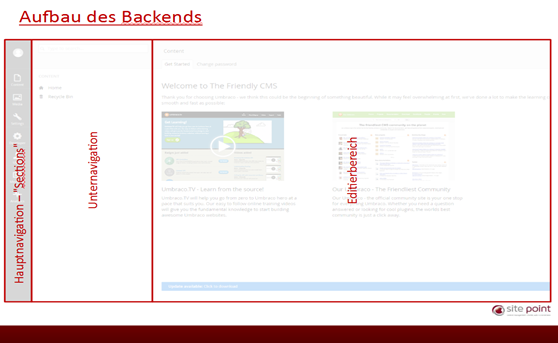
\includegraphics[width=1\linewidth]{Graphics/UmbracoBackend.png}
	\caption[Umbraco Backoffice]{Übersicht vom Umbraco-Backoffice\\Quelle: Script 11 von .NET Webkonzepte und Werkzeuge - Thomas Beckert}
	\label{fig:Umbraco Backoffice}
\end{figure}

\pagebreak
\section{Paket A}
Um der Auftraggeber mehr Flexibilität zu haben, die Frontend-Seite zu editieren, werden "Grids" - Rahmen verwendet. Grid enthält zwölf Spalten. Man kann diese Spalten zusammen binden. Auf diesem Grund es ist Möglich, die Seite auf beliebige Teilen verteilt zu werden, wie im Abbildung \ref{fig:GridsLayout} gezeigt wird.

\begin{figure}[h]
	\centering
	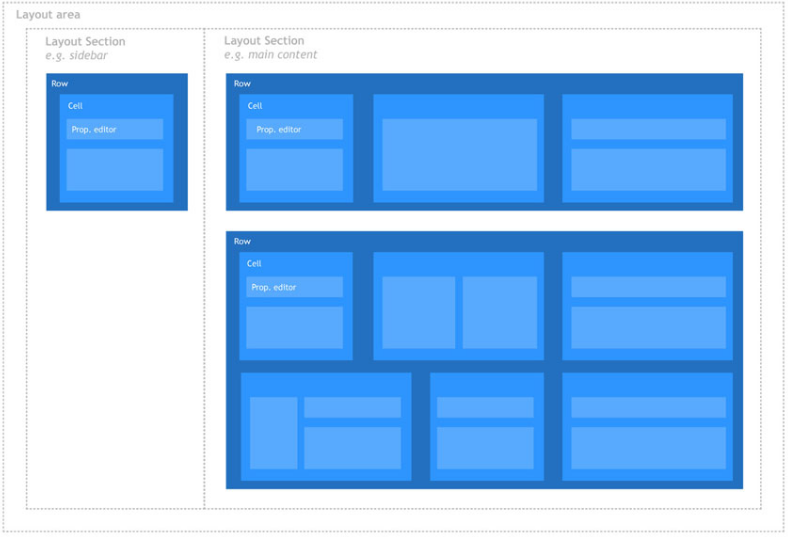
\includegraphics[width=1\linewidth]{Graphics/GridsLayout.png}
	\caption[GridsLayout]{Übersicht vom Umbraco-Grids}
	\label{fig:GridsLayout}
\end{figure}

 Im Grid kann man eigene Einstellungen machen. In dieser Arbeit werden nur zwei Beispielen gezeigt, wie Grids verwendet werden könnten- die Farbe und die Größe vom Schrift ändern. Für angefordertes Ziel werden Rich text editor und Macros verwendet. Man kann Macros auch im Rich text editor implementieren. Das wird im späteren Kapitel gemacht werden. Jetzt werden nur die bereits erwähnte Beispiele betrachtet. Sie werden im Stylesheets unter "rte" eingegeben. Im Abbildung \ref{fig:StylingGrind} kann man sehen wie CSS-Befehle im Umbraco geschrieben werden können.
     
     \begin{figure}[h]
     	\centering
     	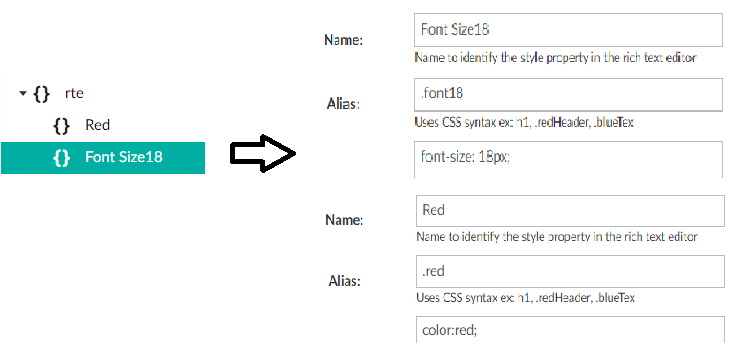
\includegraphics[width=0.6\linewidth]{Graphics/StylingGrind.png}
     	\caption[StylingGrind]{Styling vom Umbraco-Grids}
     	\label{fig:StylingGrind}
     \end{figure}
     
Über Rich text editor kann man den Inhalt des Frontends ebenfalls editieren werden, aber nur mit festen Optionen. 
Diese Stylesheet sind im Richtext edior integrierbar, somit kann der Auftraggeber die Schriftart und Farbe ändern. In der Abbildung \ref{fig:schriftManip} ist der Schrift auf rote Farbe und Größe 18pt geändert.

 \begin{figure}[h]
	\centering
	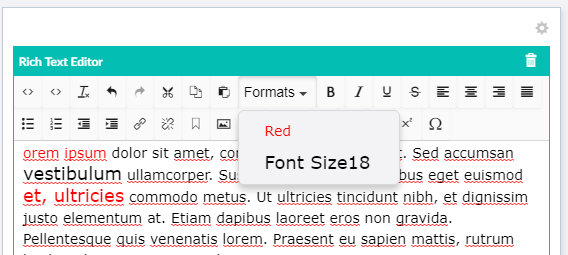
\includegraphics[width=0.6\linewidth]{Graphics/schriftManip.png}
	\caption[StylingGrind]{Styling in Umbraco-Grids - Rich text editor}
	\label{fig:schriftManip}
\end{figure}

\section{Paket B}

\subsection{Kundenverwaltung}
Die Kundenverwaltung fasst den ganzen Bereich um, der sich um die Kunden bezieht. Mehr wird es in nächster Unterkapitel erfahren.

\subsubsection{Kundenerfassung}

1. Die vorgegebene Bedingungen für diesen Bereich fassen Registrierung und Anmeldung um. Nach wie vor kann sich der Kunde anhand einer \ac{PIN} und seiner E-Mail Adresse zu dem System anmelden. Diese PIN wird automatisch generiert und  wird nach einer Bestätigung zur E-Mail des Kunden gesendet. Es muss beachtet werden, dass die E-Mail geprüft werden, ob sie sich bereits in dem Register befindet. Es wird dazu angefordert, dass der Auftraggeber den Antrag des Kunden bestätigen kann. Nach der Bestätigung kann der Kunde sich anmelden und dort kann in seiner privaten Seite des Websystems verwalten. Die Funktionalitäten bleichen mit dem alten System gleich.
Die Kundenverfassung wird durch Member-\ac{API} von Umbraco realisiert. 
Über „MemberService“ ist MemberAPI erreichbar.Diese Bibliothek ist in den Services\cite{UmbracoHQ2018Services} property von dem SurfaceController \cite{UmbracoHQ2018SurfaceController} zu Verfügung gestellt. 
Die Registrierung wird via ASP.Net Code und Media API programmatisch erstellt. Das ist eine komplexe Methode, in der vielfältige Dateien benötigt werden: (SurfaceController, Model\cite{UmbracoHQ2018Models}, PartialView und Source Datei, in der View-Methoden über eine Aufruf-Funktion aufgerufen wird). Die benötige Information, die wir zu der Registrierung brauchen, wird im Model- Datei geschrieben. 
In der Datei Model stehen Model Properties. Das sind Parametern, mit denen man arbeitet. Einfach erklärt, über das Model werden die Properties von Partial-View zu dem SurfaceController oder umgekehrt übertragen.
SurfaceController ist der „Autobahn“ zu der Umbraco-Datei. Das ist ein \ac{MVC}, das mit dem Umbraco interagiert wird. Es wird von der Bibliothek Umbraco.Web.Mvc.SurfaceController geerbt. 
Über PartialView werden die Verbindungen zwischen Kontakt Formular und Model Properties geschehen. Das ist eigentlich eine Teilansicht, die von Umbraco Frontend benutzt wird. Dort ist Umbraco \ac{UI}. 
Folgende Abbildung \ref{fig:Registrierung} ergibt bessere Verständnis wie die obengenannten Begriffe zu einander stehen.

\begin{figure}[h]
	\centering
	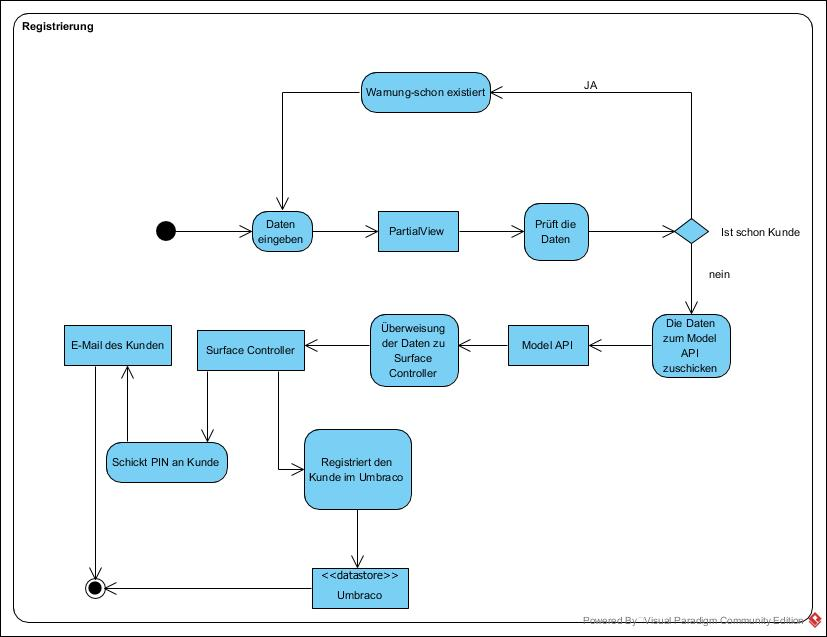
\includegraphics[width=1\linewidth]{Graphics/Registrierung.JPG}
	\caption[neues Konzept: Registrierung]{Neues Konzept zum Registrieren}
	\label{fig:Registrierung}
\end{figure}

Diese Möglichkeit vom Umbraco erlaubt den Benutzer sehr leicht und bequem in dem Server anzumelden oder sich zu registrieren.
In Anhang - Kundenerfassung kann man sich übersichtlicher genau anschauen, was es genau gemacht wird, damit diese Anforderung erfüllt wird.

\subsubsection{Kundeansicht}
Für Erleichterung des Kunde stehen auf einer Seite alle Möglichkeiten, die der Kunde hat: 

\begin{itemize}	
	\item Neue Bestellungen abgeben, aktuelle und vorherige Bestellungen ansehen
	\item Neue Nachricht schreiben und alte Nachrichten ansehen.
	\item Wichtige Information zu beachten
	\item Individuelle Information vom Auftraggeber.
\end{itemize}
1. Der Kunde bekommt einen PIN an seinem E-Mail. Die Listings \ref{lst:PINgenerator} und \ref{lst:EmailSchicken} ermöglichen den PIN, obwohl er vom Kunde nicht eingegeben wurde, direkt zur Kundes E-Mail zugechiskt zu werden.

\begin{lstlisting}[caption={JavaScript PIN Generator}, label=lst:PINgenerator]
function myFunction() {
document.getElementById('newInput').setAttribute('Value', Math.floor((Math.random() * 9000) + 1000));
}window.onload = myFunction;
\end{lstlisting}


2. Nach der Registrierung sieht der Kunde eine neue Seite. Dort kann er die obengenannten Optionen verwenden. 
Wenn der Kunde neue Bestellung tätigen will, wird ein neues Fenster geöffnet, in dem er erwünschten Artikeln wählen und bestellen kann. Die gewählten Produkte werden in den Datenbanken gespeichert. Von dort werden sie als vergangene Bestellungen verwendet. Das selben Prinzip steht auch für die Kommunikation zwischen den Auftraggeber und den Kunden. Wenn eine Nachricht geschrieben wird, wird sie in den anderen Datenbanken gespeichert. 
Vom Umbraco wird die Information direkt zu den Kunden gesendet. 
Der Auftraggeber, so wie der Kunde, können von der Datenbank die Bestellungen und die Nachfragen ansehen. In den weiteren Kapitel wird detailliert erklärt wie die Kommunikation und die Aufträge funktioniert.
3. Nach angefordertes Ziel wird den Kunde Profile-Seite über Member abgebildet. Das Bedeutet, dass diese Seite ist nur zum jeweiligen Kunde personalisiert. Die Abbildung wird über memberId geschehen. Es wird ein Filter erstellt, durch das diese Personalisierung erreichen wird. memberId befindet sich im umbraco-Member Datenbank.
Das, was im Kundenansicht gemacht wurde, ist Verwendung von Macros und Grids. 
Damit man besser versteht, worum es geht, wird folgenden Abbildung \ref{fig:kundenansichtNew} erstellt. 

\begin{figure}[h]
	\centering
	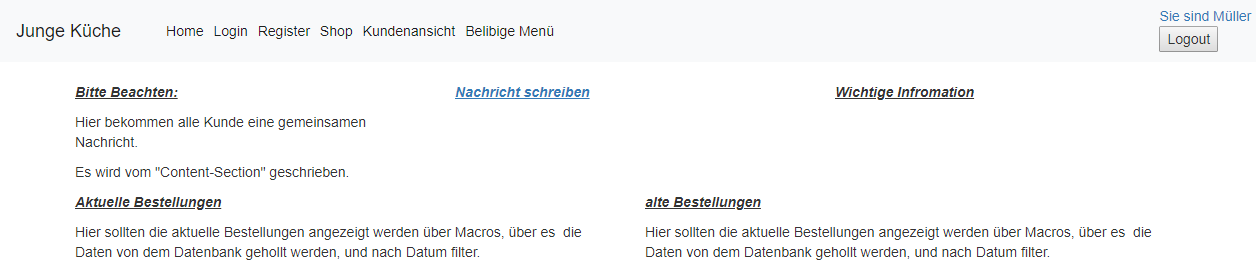
\includegraphics[width=1\linewidth]{Graphics/kundenansichtNew.png}
	\caption[Kundeansicht]{Kundeansicht}
	\label{fig:kundenansichtNew}
\end{figure}
Über ein Macros, das man im Listing \ref{lst:macroKundenansicht} anschauen kann, ist es Möglich die Meldungen vom Auftraggeber unter "Wichtige Information"  zu sehen. Im Macro ist eine Methode schrieben, über sie wird die Übertagung vom Member-Section zum Content-Section ermöglicht wird. Abbildung \ref{fig:kundenansichtNew} zeigt, wie der Auftraggeber zu dem Kunde eine Informationsmeldung von Member-Bereich schickt.
\begin{figure}[h]
	\centering
	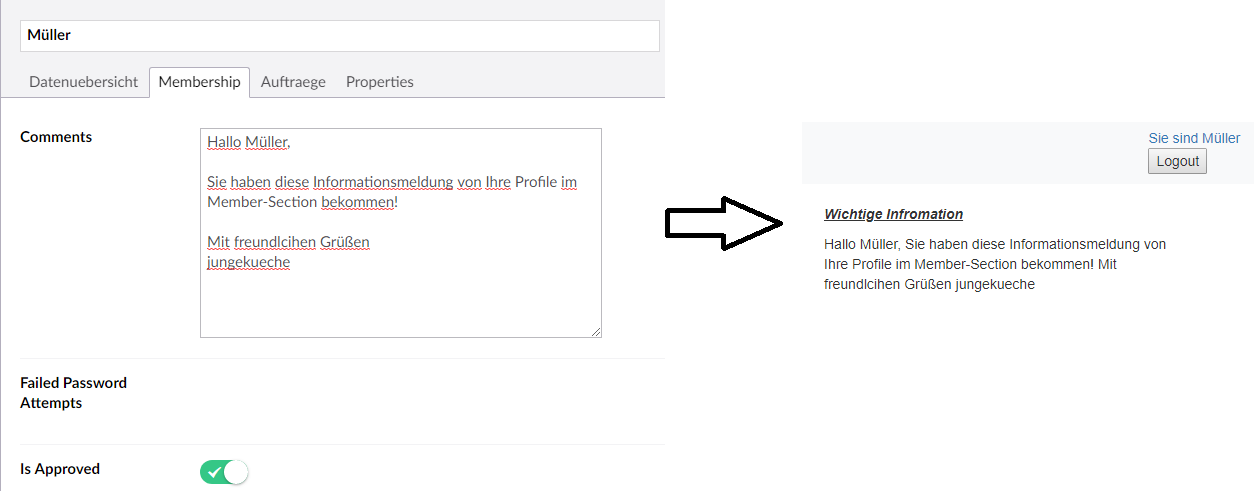
\includegraphics[width=1\linewidth]{Graphics/kundenAnsichtWichtInf.png}
	\caption[Kundeansicht]{Übertragung der Informationsmeldung von Member-Section zu Kundenansicht}
	\label{fig:kundenAnsichtWichtInf}
\end{figure}
\pagebreak
\begin{lstlisting}[caption={Macro zum Kundenansicht}, label=lst:macroKundenansicht]

@inherits Umbraco.Web.Macros.PartialViewMacroPage


@{
	var memberID = ApplicationContext.Current.Services.MemberService.GetByUsername(Membership.GetUser().UserName);
	var info = memberID.Comments;
}
@info
\end{lstlisting}

Das Kontaktfenster und allgemein die Bestellungen werden im weiteren Unterkapitel erläutert. Das gesamte Bild wird im Abbildung \ref{fig:KundenansichtNeu} dargestellt.

\begin{figure}[h]
	\centering
	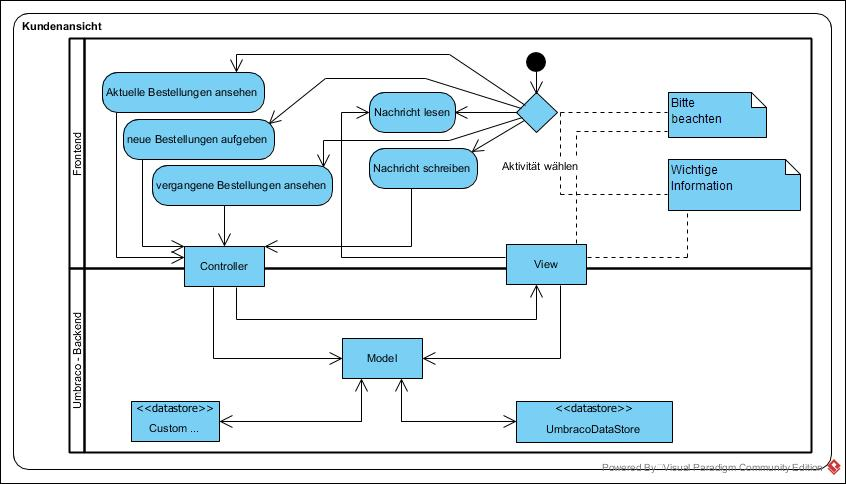
\includegraphics[width=1\linewidth]{Graphics/KundenansichtNeu.jpg}
	\caption[Funktionalität von Kundenansicht]{Funktionalität von Kundenansicht}
	\label{fig:KundenansichtNeu}
\end{figure}

\subsubsection{Auftraggeber-Ansicht}
  
1. Mithilfe vom Umbraco-Member-Section kann der Auftraggeber seine Kunde filtern. Es gibt eingebaute Einstellungen, wie ListView \cite{UmbracoTV2018ListView}. Durch diese Möglichkeit ist man kann die Kunden im Member-Bereich filtern, nach dem Name suchen oder löschen. Es kann auch zusätzliche Properties erstellt werden. Diese Properties können über extra Attribut im Model-Datei mit dem Frontend verbunden werden.
Hier wurden neuen Tabs und Properties srtellt. Als Beispiele wird Tab-"Datenuebersicht" gegeben. Dort befindet sich nur ein Property "Ort". Im Tab-Membership ist "Password" auch ein Beispiel, aber man kann mehrere einbauen. Abbildung \ref{fig:auftraggeberAnsichtDaten} stellt dieses Tab und zugehöriges Property dar.

\begin{figure}[h]
	\centering
	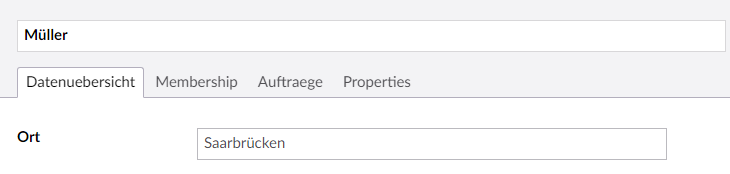
\includegraphics[width=1\linewidth]{Graphics/auftraggeberAnsichtDaten.png}
	\caption[Kundeansicht]{Beispiel zur Erstellung eines extra Tab und Property}
	\label{fig:auftraggeberAnsichtDaten}
\end{figure}
 Wie schon erläutert wurde, ist ein Macro erstellt, durch das die Information zum jeweiligen Kunde Zugeordnet ist. 

Um die Migration problemlos durchgeführt zu werden, muss man eine neue Zuordnung im Member-Bereich realisieren. Die neue Properties müssen zu den alte übertragene Attributen von der Member-Datenbank zustimmen. Mehr dafür wird im Unterkapitel "Übersicht" erläutert.  
\subsubsection{Kommunikation}

In diesem Kapitel wird beschrieben, die Kommunikation zwischen dem Auftraggeber und dem Kunde. Als Anforderung wird eine Übersichtliche Kommunikationsmethode mit Filtern (gelesen, nach Kunden suche...) festgestellt.

Es wird ContentAPI \cite{UmbracoHQContent2018} verwendet. In Kundenansicht wird über ein View Nachricht-Form, damit der Kunde Nachrichten schicken kann. Mithilfe der Model und SurfaceController die Nachricht wird in der Umbraco Conten-Section. Dort sie wird als neue Untertreenode im vorgemachte Tree "Nachrichten" Dieses Tree wird mithilfe von Umbraco-ListView modelliert. Umbraco-ListView ermöglicht beliebig viele Untertreenodes, in einem einzigen Tree gelagert zu werden. Um die Nachrichten zu dem zugehörigen Kunde zu stimmen, wird es in jeweilige Nachricht das IDnummer des Kunden integriert. Mithilfe diesem Nummer wird es möglich auch ein Filter aufgebaut. Somit kann die Kunde nur seine private Nachrichten lesen. Listings \ref{lst:NachrichController} und Abbildungen \ref{fig:NachrichtNEU} und \ref{fig:NachrichtUmbraco} zeigen den ganzen Verlauf der Kommunikation.

\begin{figure}[h]
	\centering
	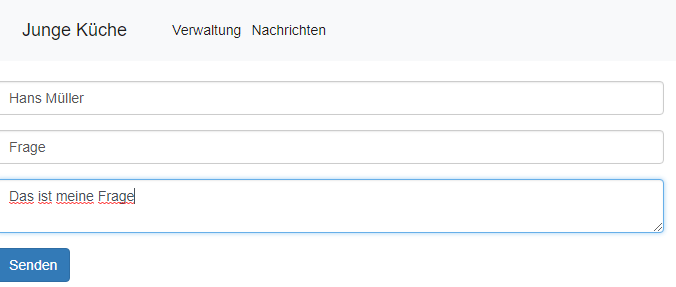
\includegraphics[width=0.7\linewidth]{Graphics/NachrichtNEU.png}
	\caption[Nachricht Formular]{Nachricht Formular}
	\label{fig:NachrichtNEU}
\end{figure}
\begin{lstlisting}[caption={NachrichController}, label=lst:NachrichController]

namespace newKonzept.Controllers.NachrichtController
{
public class NachrichtController : SurfaceController
{
// GET: Nachricht
public ActionResult Index()
{
return PartialView("NachrichtPartial/NachrichtPartial", new NachrichtModel());
}
[HttpPost]
public ActionResult HandleFormSubmit(NachrichtModel model)
{
if (!ModelState.IsValid)
{
return CurrentUmbracoPage();
}

var memberID = ApplicationContext.Current.Services.MemberService.GetByUsername(Membership.GetUser().UserName);
model.SenderId = memberID.Id;
var comment = Services.ContentService.CreateContentWithIdentity(model.Sender, CurrentPage.Id, "nachricht");

comment.SetValue("Betreff", model.Betreff);
comment.SetValue("Sender", model.Sender);
comment.SetValue("Message", model.Message);
comment.SetValue("SenderId", model.SenderId);

Services.ContentService.Save(comment);

Services.ContentService.Save(comment);
TempData["success"] = true;

return RedirectToCurrentUmbracoPage();
}
}
}
\end{lstlisting}


\begin{figure}[h]
	\centering
	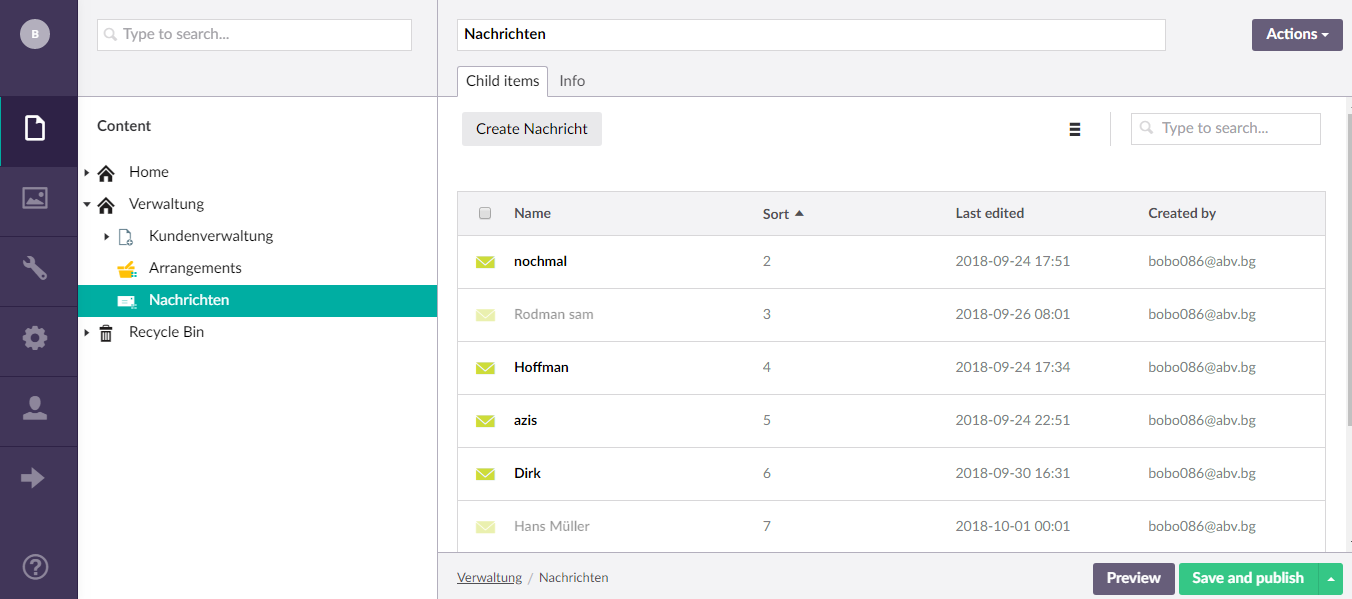
\includegraphics[width=0.7\linewidth]{Graphics/NachrichtUmbraco.png}
	\caption[NachrichtUmbraco]{Nachricht in Umbraco-Backoffice}
	\label{fig:NachrichtUmbraco}
\end{figure}

Wenn die Nachricht nicht gelesen ist, ist durchsichtig. In dem geöffneten Fenster, steht die gesendete Nachricht. Neben dran ist "Antwort"-Tab. Somit kann der Auftraggeber die Frage beantworten. Die Nachrichten werden nach memberID gefiltert. In Abbildung \ref{fig:Message} und \ref{fig:antwort} wird die Rückfrage dargestellt.

\begin{figure}[h]
	\centering
	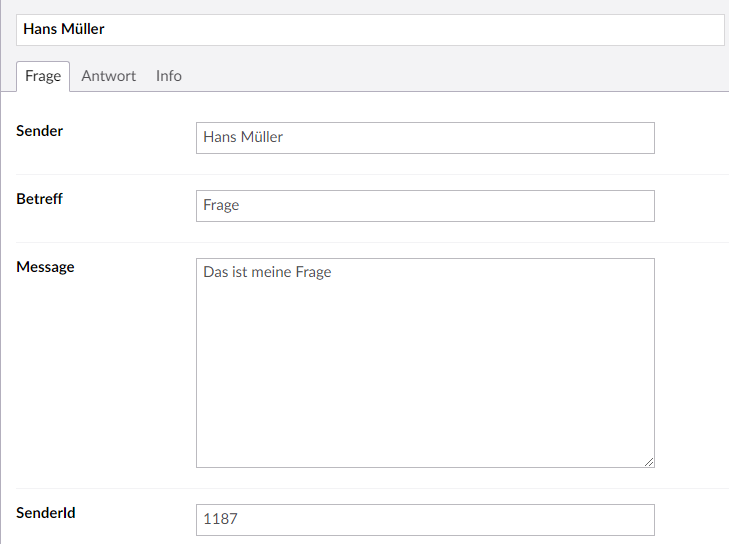
\includegraphics[width=0.7\linewidth]{Graphics/Message.png}
	\caption[Nachricht]{Die Nachricht wurde bekommen}
	\label{fig:Message}
\end{figure}

\begin{figure}[h]
	\centering
	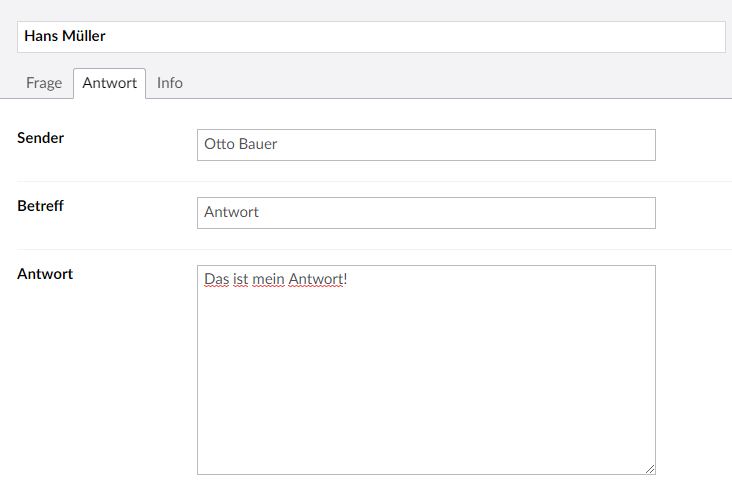
\includegraphics[width=0.7\linewidth]{Graphics/antwortMassege.png}
	\caption[Nachricht]{Antwort Schreiben}
	\label{fig:antwort}
\end{figure}

\pagebreak

In Listing ist das Filter, das in einem Macro integriert wird, dargestellt.

\begin{lstlisting}[caption={NachrichFilter}, label=lst:NachrichFilter]

<ul>

@foreach(var item in selection){

var pageId = item.GetPropertyValue
<string>
("senderId");
if(pageId.ToString() == memberID.Id.ToString()){
<li>
<a href="@item.Url">@item.Name</a>
</li>
}
}
</ul>
\end{lstlisting}

Der Kunde sieht die Antwort von dem Auftraggeber, wie in der Abbildungen \ref{fig:bekommen} und \ref{fig:alleNachrichten} gezeigt wird.
\begin{figure}[h]
	\centering
	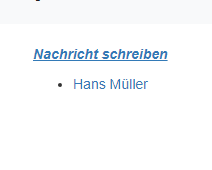
\includegraphics[width=0.3\linewidth]{Graphics/nachrichtBekomm.png}
	\caption[Nachricht]{Antwort bekommen}
	\label{fig:bekommen}
\end{figure}

\begin{figure}[h]
	\centering
	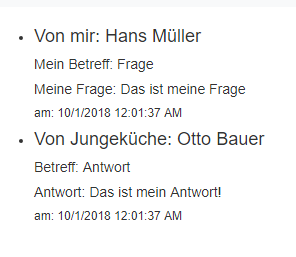
\includegraphics[width=0.3\linewidth]{Graphics/dialog.png}
	\caption[Nachricht]{Alle Nachrichten}
	\label{fig:alleNachrichten}
\end{figure}
 
 \pagebreak
 
\subsection{Artikelverwaltung}

\subsubsection{Erfassen, editieren und löschen}

In der vorgegebenen Aufgabe muss den Online-Editor mit zwei Kategorien sein - Arrangements und Artikel-Standard. Diese müssen zu den zugehörigen Webseiten gekoppelt werden. Als Anforderung steht, dass Artikel-Verwaltung einfacher verwaltet werden kann und die Artikelseite der Webseite soll direkt mit dem Artikel gekoppelt sein. In der alten Seite ist die Artikel-Verwaltung nicht mit den zugehörigen Seite gekoppelt. Migration ist nicht angefordert.

Das betrachtete Ziel wird über Macros, PetaPoco-Datenbank \cite{Robinson2018} und Umbraco vorgegebene Funktionen. Zuerst wird Umraco ListView verwendet, damit die erstellte Artikel sich im Umbraco-Content-Section unter einer gemeinsamen Unteroption befinden. Dazu ist auch vorgegeben, dass den neuen erstellten Artikel direkt editiert werden kann. Abbildung \ref{fig:ArtikelVerwaltung} zeigt übersichtlicher wie die Artikel-Verwaltung aussieht.

\begin{figure}[h]
	\centering
	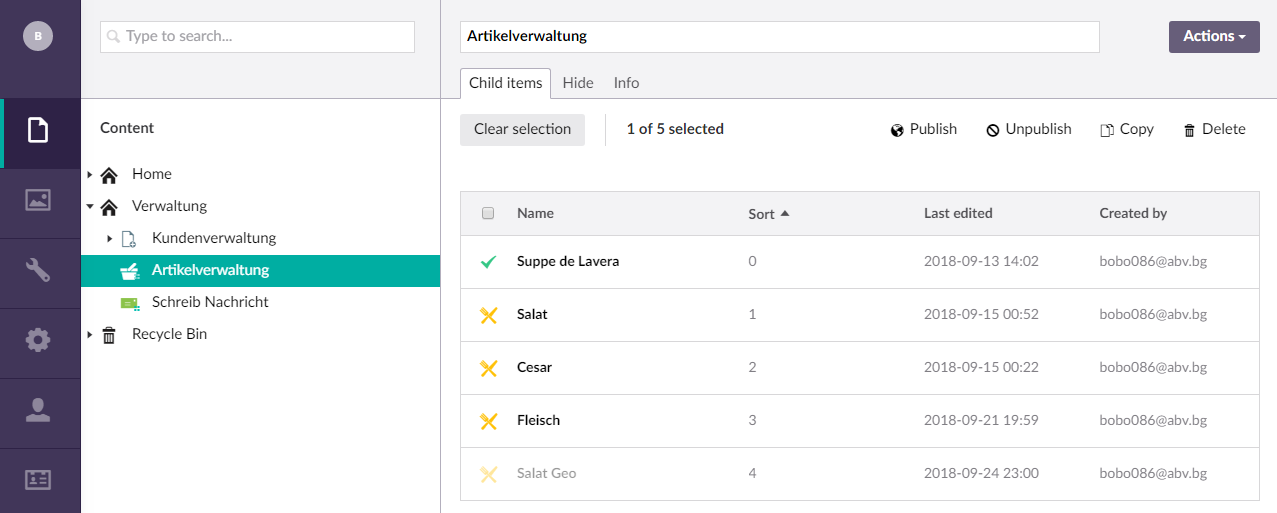
\includegraphics[width=1\linewidth]{Graphics/ArtikelVerwaltung.png}
	\caption[ArtikelVerwaltung]{Übersicht der Artikel-Verwaltung}
	\label{fig:ArtikelVerwaltung}
\end{figure}

Wenn der Artikel "unpublish" ist, kann er nicht im Frontend verwendet wird. Wenn die Artikel schon erstellt sind, wird ein Quellcode im Macros programmiert. Diese Macros werden im schon besprochenen Grids integriert, über die die Inhalt der Artikel zum Frontend übertragen wird. 
Die Inhalt wird nicht nur mit den Webseiten, sonder auch mit dem Shop-Menü gekoppelt. So wird Selbständigkeit des Auftraggeber verbessert. In der nächsten Abbildung wird gezeigt, wie mit der Erstellung von einem Artikel, werden seinen Daten sowohl im zugehörige Seite, als auch in der Shop-Menü gekoppelt.
 
Wenn der Kunde registriert ist, kann er die von dem Auftraggeber eingegebene Artikel aus dem Shop wählen. Nach der Bestellung werden die Daten in der Datenbank "Artikel" gespeichert. Gleichzeitig werden diese Daten zusammen mit dem Kunden Daten auch im Datenbank "Auftraege" gespeichert. Aus Abbildung \ref{fig:Shop} wird gesehen, dass die Daten von der Artikelverwaltung wurden erfolgreich zu dem Shop versendet.

\begin{figure}[h]
	\centering
	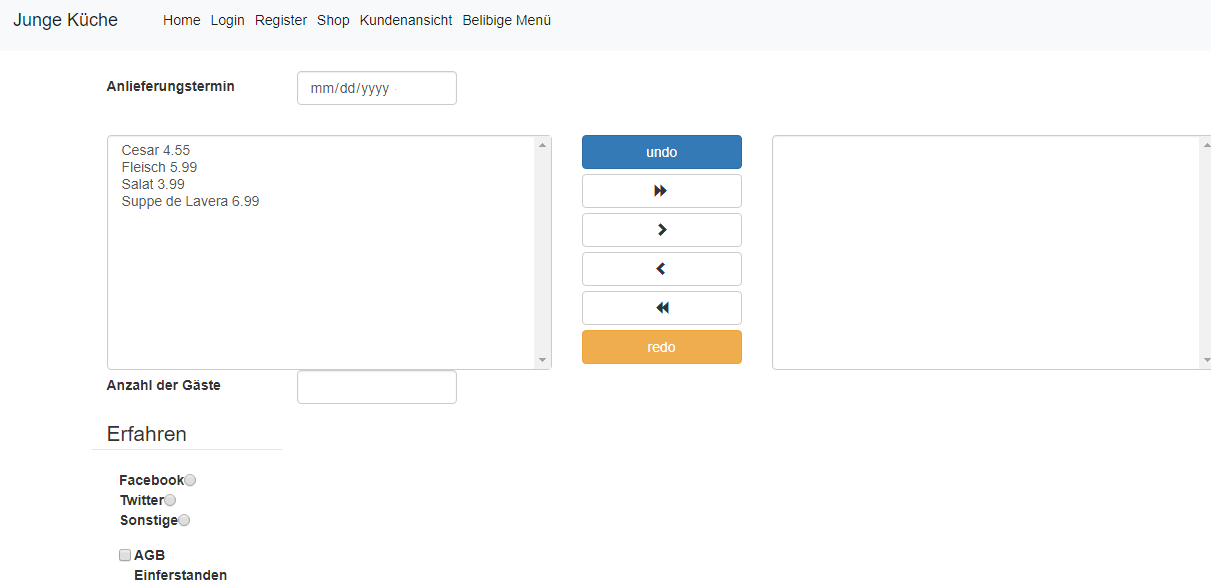
\includegraphics[width=1\linewidth]{Graphics/shop.png}
	\caption[Shop]{Übersicht des Shops}
	\label{fig:Shop}
\end{figure}


\subsection{Auftragsverwaltung}

\subsubsection{Übersicht}

Das vorgegebene Ziel ist eine Übersicht über die Aufträge und Nachrichten. Diese Ansicht soll in einer eigenen Umbraco-Section umgesetzt werden. Die Artikeldatenbank soll von Access nach SQL transportiert werden. Es muss eine neue Zuordnung zu Umbraco-Member geben.

Das vorgeschlagene Konzept umfasst die Migration von Access Datenbankdatei und Erstellung von neue Custom-Section. 

1. Um ein neues Section aufgebaut zu werden, braucht man zuerst in einer Klasse-Datei, Methoden von den Bibliotheken "umbraco.buisnesslogic" und "umbraco.interfaces" aufzurufen. Über "Application"-Methode und "IApplication"-Interface. Somit wird die Custom-Section erstellt. Wenn das fertig ist, wird die Übersicht über AngularJS-Controller und HTML erstellt. Diese Dateien werden zu dem API-Controller über Paket-Manifest referenziert. In diesem Controller werden die eigentliche Funktionalitäten von Custom-Section realisiert. Mithilfe dem API-UmbracoAuthorizedJsonController werden die Daten über Model-Attributen von schon erstellter Datenbank "Auftrage" zur Verfügung gestanden, die schon im vorherigen Unterkapitel erwähnt wurde. Die Datenbanken werden über PetaPoco erstellt. In der Abbildung \ref{fig:CustomSection}  stellt die Kommunikation dar. 
 
 \begin{figure}[h]
 	\centering
 	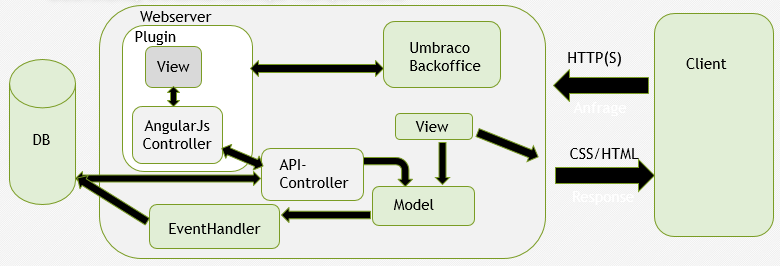
\includegraphics[width=1\linewidth]{Graphics/CustomSection.png}
 	\caption[Shop]{Eine Übersicht von Kommunikation zwischen verschiedene Elemente}
 	\label{fig:CustomSection}
 \end{figure}
 
2. Wie es angefordert wurde, soll eine Migration von Access-Datenbank zu Umbraco durchgeführt werden. Das angestrebte Ziel ist, dass die alten Daten in der neuen zugehörigen Datenbank gespeichert werden. Die neue betrachtete Datenbanken sind Custom-"Artikel" und "Umbraco-Member". 
Nach tiefer Recherche wird ein Konzept erstellt. 
Grundsätzlich stehen im Umbraco Member-Section \cite{OurUmbraco2018} drei Unteroptionen - Members, Member Types und Member Groups.
Im Member Type wird die Einstellungen (Properties) des Members aufgebaut. Dort wird eine neue Member Type mit extra Properties erstellt. 
Folgendes Konzept ist basiert auf der Erwartung, dass die Datenbanken von Access auf CSV-Format konvertiert sind. Das Bedeutet, dass die Accsess-Datenbankformat Datei auf einer Text-Datei umgewandelt wird. Somit kann man die Methode StreamReader nutzen.
Um das vorgegebene Ziel realisiert zu werden, braucht man, ein SurficeController zu erstellen, das die Übertragung leitet. 
Umbraco verfügt mit spezielle "Autobannen", durch die möglich ist die Manipulation von festgelegte Sections im Umbraco. Man nennt diese "Autobannen" - "Services". Sie werden über ApplicationContext aufgerufen. In diesem Fall wird "MemberService" genutzt.
Damit die Datei gelesen wird, wird die Funktion StreamReader verwendet. Somit wird die gelesene Datei in einer Variablen gespeichert. Von dieser Variablen wird mithilfe von dem Befehl-split in einem Array gespeichert. Jeder Teil von dem Array wird über MemberService Befehle und Methoden im Umbraco Members gespeichert. Im Anhang \ref{lst:migrationsController} steht das Quellcode, um man besseres Vorbild zu haben, sowie in der Abbildung \ref{fig:DBMigration} für eine klare Übersicht der Migration dargestellt wird.

 \begin{figure}[h]
	\centering
	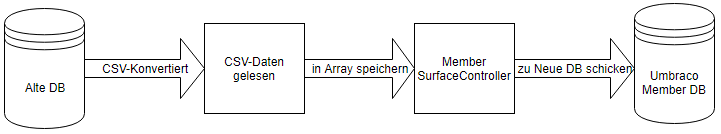
\includegraphics[width=1\linewidth]{Graphics/DBMigration.png}
	\caption[Shop]{Eine Übersicht von Kommunikation zwischen verschiedene Elemente}
	\label{fig:DBMigration}
\end{figure}

Wenn die Kundendaten schon übertragen wurden, kann man das selben Prinzip der Migration für die Artikel benutzen. Hier wird als Ziel statt MemberServices - Datenbank Artikel-Datenbank  verwendet. Nach der Umwandlung von Access-Datenbankdatei auf CSV-Format, wird diese Datei über die Methode StreamReader, danach ist die Information im ein Array gespeichert. Über API-Controller werden die Daten im "Artikel"-Datenbank übertragen. In Listing \ref{lst:DBInputArtikel} wird anschaulicher gesehen, wie läuft die Übertragung der Daten durch. 

\begin{lstlisting}[caption={Datenbank "Artikel" - Transfer}, label=lst:DBInputArtikel]

var setArtikel = new Artikel();
var db = new PetaPoco.Database("umbracoDbDSN");
setArtikel.kundeID =_split[0];
setArtikel.bezeichnung = _split[1];
setArtikel.beschreibung = _split[2];
setArtikel.preis = _split[3];
setArtikel.art = _split[4];
setArtikel.kannWaehelen = m_split[5];

db.Insert(setArtikel);
\end{lstlisting}

\subsubsection{Detailansicht}

Hier wird angefordert, dass der Auftraggeber die Aufträge bearbeiten kann, den Status ändern, Positionen editieren, hinzufügen oder löschen, dem Kunden Freigaben erteilen (zum Beispiel Aussuchen der Positionen) und ein Rechnungsnummer vergeben. Diese Aktivitäten sind gleich mit der alten Webseite und müssen in eigenem Umbraco-Section umbesetzt werden. 

Die Erstellung von dem Custom-Section ist bereits bekannt. Hier wird es mit den Auftraege- und Member-Datenbank über AngularJS-Controller anhand des Package-Manifest zu dem API-UmbracoAuthorizedJsonController verbunden. In Listings \ref{lst:AngularJS} und \ref{lst:API-Controller} wird gezeigt wie die Daten von der Datenbank aufgerufen werden.

\begin{lstlisting}[caption={AngularJS-Controller ruft die zugeordnete Methoden im API-Controller}, label=lst:AngularJS]

angular.module("umbraco").controller("Detailansicht.editController", function ($scope, $routeParams, auftragResource, navigationService, notificationsService) {

	$scope.loaded = false;

	// Inhalt wird geladen
	if ($routeParams.id == -1) {
		$scope.auftrag = {};
		$scope.loaded = true;
	}
	else {
	// Artikel wird geladen
		auftragResource.getById($routeParams.id).then(function (response) {
		$scope.auftrag = response.data;
		$scope.loaded = true;
		});
	}

	$scope.save = function (auftrag) {
		auftragResource.save(auftrag).then(function (response) {
		// $scope.auftrag.$isdirty = false;
			$scope.auftrag = response.data;
			notificationsService.success("Success", auftrag.auftragId + " " + " has been saved.");
			navigationService.syncTree({ tree: 'auftragTree', path: [-1, $scope.id], forceReload: true }).then(function (syncArgs) {
				navigationService.reloadNode(syncArgs.node);
				});
			});
	}
});
\end{lstlisting}

\begin{lstlisting}[caption={API-UmbracoAuthorizedJsonController}, label=lst:API-Controller]

namespace newKonzept.Controllers.DB
{
	[PluginController("Detailansicht")]
	public class AuftragApiController : UmbracoAuthorizedJsonController
	{
		private Database db = new Database("umbracoDbDSN");
		public IEnumerable<Auftraege> GetAll()
		{
			List<Auftraege> liste = new List<Auftraege>();
			foreach (Auftraege auftrag in db.Query<Auftraege>("SELECT * FROM Auftraege"))
			{
				liste.Add(auftrag);
			}
			return liste;
		}
	public Auftraege GetById(int id)
	{
		return db.SingleOrDefault<Auftraege>("SELECT * FROM Auftraege WHERE auftragId=@0", id);
	}

	public Auftraege PostSave(Auftraege auftrag)
	{
		if (ModelState.IsValid)
		{			
			if (auftrag.auftragId > 0)
			{
				db.Update(auftrag);
			}
			else
			{
				db.Insert(auftrag);
			}
		}
		return auftrag;
	}

	public int DeleteById(int id)
	{
		var db = new PetaPoco.Database("umbracoDbDSN");
		return db.Delete<Auftraege>("WHERE auftragId=@0", id);
	}
}
\end{lstlisting}

Die Daten von Member-Datenbank werden als String über MemberService aufgerufen und in ein Array gespeichert. Dieses Array wird von der AngularJS aufgerufen und zu HTML-Plugin-Editor zugeschickt. Die Daten des Members können in der Detailansicht nicht geändert werden, deswegen werden sie als String verwendet.